%!TEX root = ../template.tex
%%%%%%%%%%%%%%%%%%%%%%%%%%%%%%%%%%%%%%%%%%%%%%%%%%%%%%%%%%%%%%%%%%%%
%% chapter3.tex
%% NOVA thesis document file
%%
%% Chapter with a short laext tutorial and examples
%%%%%%%%%%%%%%%%%%%%%%%%%%%%%%%%%%%%%%%%%%%%%%%%%%%%%%%%%%%%%%%%%%%%
\chapter{State of the Art}
\label{cha:state_of_the_art}

This Chapter aims at detailing data sources in the farming field, previous works done in this field of study, their pros and cons, limitations and viability in the FitoAgro project.

\section{Data from the field} % (fold)
\label{sec:state_of_the_art_data}


Collecting data from field and building a complete digital model of the plot is not an easy task. Several variables come into play and problems such as connectivity, low to none maintenance and cost of the equipment arise. These requirements may condition the amount georeferenced data-sources, their efficiency, resolution, autonomy, etc.

Revisiting the methodology of Precision-Agriculture, data-collection is probably the most important step in this 4-step process. In order to be able to calculate pest and disease regional economic risk levels, weather information needs to be available for indiviual fields(shapes). Hopefully, in the future, measures from different fields can be analised together in a continuous mesh including several fields as described in \cite{Ojha2015}. Different sampling points have to be spread across the region of study in order to build a map. This is not directly helpful to the farmer, since he mainly cares about his fields, but may help to better understand the behaviour of such pest species.

\subsection{Satellite Imagery}
\label{sec:satellite_imagery}

Satellite imagery is slowly becoming accessible for public use. While free satellites provide imagery with low temporal and geographic resolutions, paid services (though costly) provide very high resolutions. Multi-spectral imagery provides raw data that can be turned into temperatures, Normalized Difference Vegetation Index (NDVI), Moisture and Soil maps with resolutions up to 0.41m.

Satellite sensors deliver 16-Bit 4-Band (B,G,R,N) or 8-Band (C,B,G,Y,R,RE,N,N2) Multispectral pixel resolutions from 1.2m to 5m. Pansharpened vegetation indices can be delivered with a resolution of 30cm, 40cm or 50cm, providing greater details for analysis. 

The Sentinel-2 Satellite sensors acquires 10m 4-band (BGRN) Multispectral, 20m 4-band RedEdge and 2-band Short Wave InfraRed and 60m 3-band Coastal Aerosol, Water Vapour and SWIR Cirrus Imagery providing a choice for a good selection to search for cloud free Imagery for the Area Of Interest (AOI). This Imagery is very suitable to deliver 10m resolution NDVI or other vegetation index Imagery and moisture maps in KMZ format. Because the Sentinel-2 Satellite Imagery, provided by the European Space Agency (ESA), can be downloaded for free and requires only vegetation and soil index image processing, providing a cost effective Ag solution, covering large areas around the globe, were 10m resolution is acceptable or desired due to limited financial resources.

The satellites in the SENTINEL-2 constellation will provide a revisit time of 5 days at the equator in cloud-free conditions. The fees for Sentinel-2 produced vegetation index Imagery (NDVI, TSAVI etc.) and moisture maps are starting at US \$ 0.20\/ Ac or US \$ 0.49/ Ha for a combination of 2 vegetation indices and 1 moisture map, with a minimum commitment of 1,000 Ac or 405 Ha and 2 months of service, including the delivery of up to six (6) Sentinel-2 scenes in Natural Color and Color InfraRed (CIR), vegetation index scenes in GeoTIFF, IMG or KMZ format.

The agriculture, forestry and environmental industries have been using the standard NDVI index for many years but with the availability of hyperspectral sensors and high resolution Satellite sensors, such as WorldView-2 and WorldView-3, utilizing an expanded Multispectral reflectance range, Satellite imagery can provide a variety of vegetation indices to filter the correct band combinations for vegetation, soil and environmental analysis to support crop management.

\begin{figure}[htbp]
  \centering
  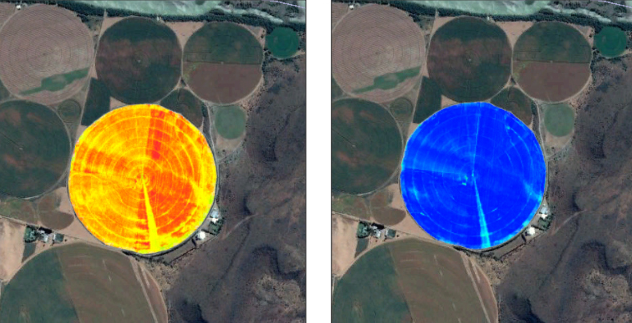
\includegraphics[width=0.9\linewidth]{worldview-2-moisture-map-ndvi}
  \caption{WorldView-2 NDVI Index (left) and Moisture Map (right) - South Africa}
  \label{fig:worldview-2-moisture-map-ndvi}
\end{figure}


WorldView-3 Satellite sensors collect in addition to the standard Panchromatic and Multispectral bands, eight-band short-wave infrared(SWIR) and 12 CAVIS imagery.\\\mbox{WorldView-3} is the first multi-payload, super-spectral, high-resolution commercial satellite sensor operating at an altitude of 617 km. WorldView-3 satellite provides 31 cm panchromatic resolution, 1.24 m multispectral resolution, 3.7 m short wave infrared resolution (SWIR) and 30 m CAVIS resolution. The satellite has an average revisit time of <1 day and is capable of collecting up to 680,000 km2 per day.

In the past, a known limitation of satellite use were clouds. In cloudy days, the area under analysis could be covered in clouds, breaking line-of-sight between the satellite and a specific land location, resulting in no readings during that portion of time. Since the revisit times were usually > 1 day (i.e. 1 reading per day), this would mean that there would be days without any readings.

Biological readings from multispectral GIS(Geographic Information System) for each of the plants is still not possible. Some recent studies have shown progress in using SWIR for optical remote detection but, using satellite imagery, the only part of the tree visible is the crown (composed by leaves, twigs and branches). The resolution of 0.31 (max resolution of the WorldView-3), even if generally considered good, is not good enough to track these micro organisms. Example of SWIR for canopy assesement in figure \ref{fig:managed-canopy-web}.

\begin{figure}[htbp]
  \centering
  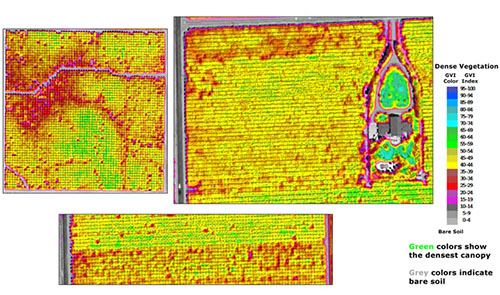
\includegraphics[width=0.9\linewidth]{managed-canopy-web}
  \caption{Managed Canopy Assessment (tree chrowns). Soils(top left), Health (top right) and Irrigation(bottom). Image from Worldview-3.}
  \label{fig:managed-canopy-web}
\end{figure}

Analysis drawn from this data-source are essentially growth indicators by vegetation indices (from reflectance and Chlorophyll), soil temperatures from shortwave infrared and irrigation if using the WorldView-3 SWIR.

In sum, there is a tradeoff between resolution/features and pricing. For agricultural use, there are no tight requirements in revisit times (temporal resolution) nor image resolution but the features from Worldview-3 in terms of Infrared analysis are revolutionary. While Short-Wave Infrared (SWIR) bands add spectral coverage to the invisible range, providing ground-breaking analysis of the land surface, CAVIS (stands for Clouds,  Aerosols, Water Vapor, Ice and Snow) corrects for the inconsistencies caused by certain conditions, offering standardized imagery no matter where or when the data was captured.

\subsection{Weather Stations}
\label{sec:weather_stations}

Weather stations provide measurements from a single location: the station location. In theory, while providing accurate readings, weather stations have initial costs and/or fixed costs (depending on the brand of the station) and maintenance is scarce due to their remote locations. In reality, most of the fields that have weather stations, their sensors are not accurate (require calibration) or completely not working.

Weather stations networks are publicly available for free but with minor issues. Data access is somewhat limited: Measurements are not available through API, and the exporting capabilities are somewhat hard to incorporate into the system

The FitoAgro project has facilitated weather stations already operating, so, to drive costs down and speed up developments on the data collection process, weather stations will be used as a starting point (with the possibility of extending and interpolation using Satellite imagery as described in \ref{sec:satellite_imagery}. Some weather stations already incorporate soil sensing capabilities, but this is obviously dependant on the brand of the equipment.

\begin{figure}[htbp]
  \centering
  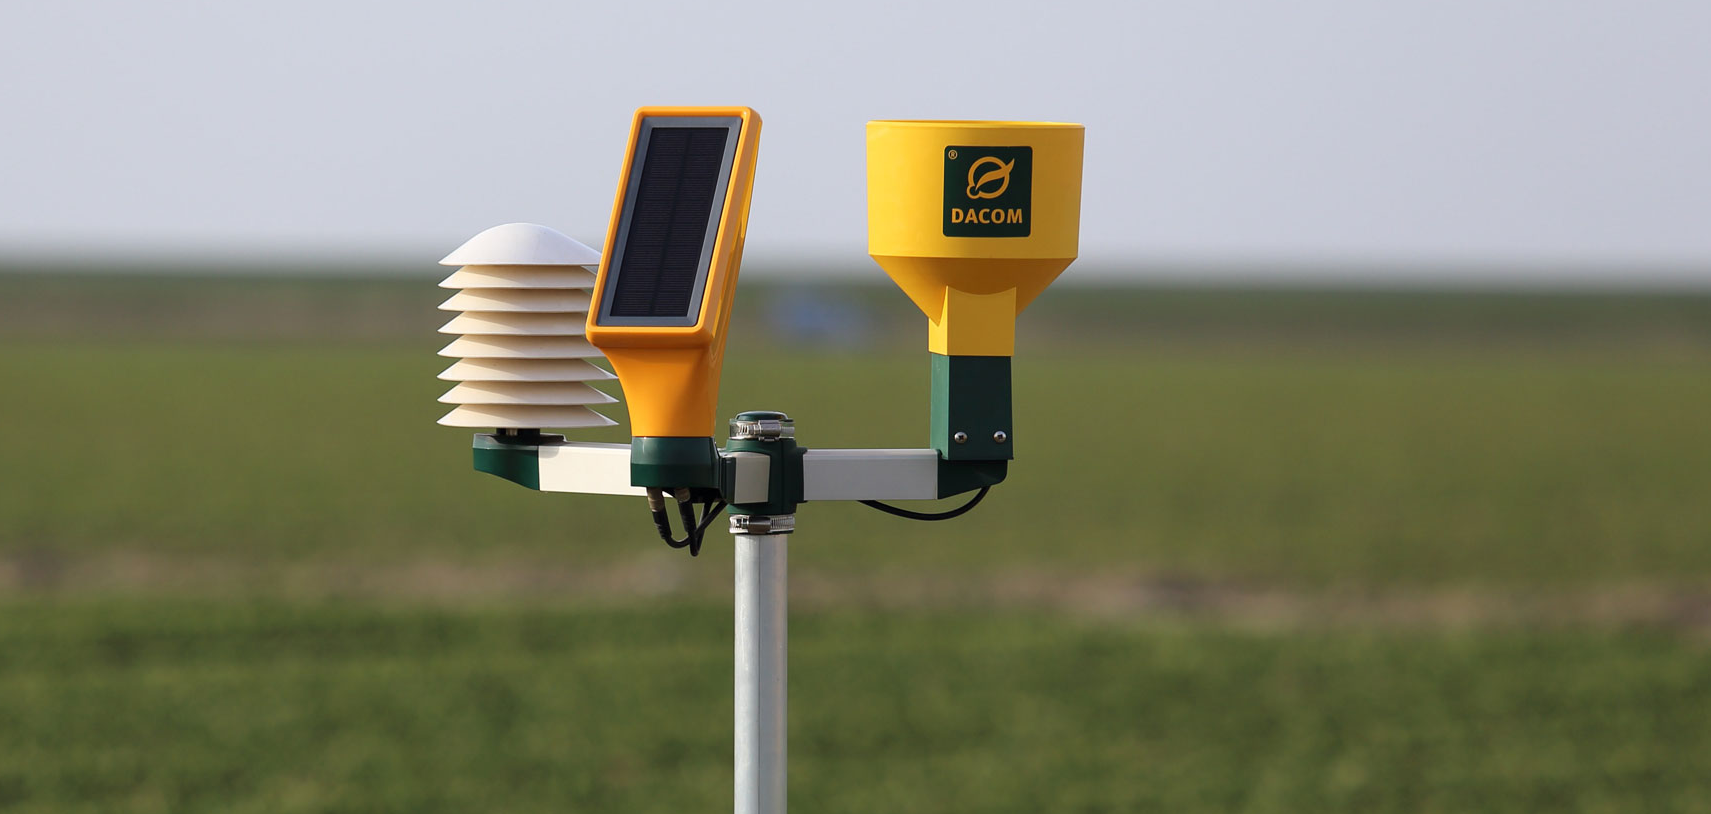
\includegraphics[width=0.7\linewidth]{weather_station}
  \caption{Simple weather station with 3 sensors: temperature, relative air humidity and rain gauge.}
  \label{fig:weather_station}
\end{figure}

The single point measurement is a problem itself: it does not provide enough data to map to the field. Two opposing corners of the same farming field will inherit the same weather and soil information since there is no way to provide better granularity using a single weather station. For the work developed in this dissertation, it is assumed that the weather variations throughout a single farming field are negligible (weather measurements not human influenced, i.e. irrigation affecting soil moisture).

In the end, the variables that we are able to gather from weather stations with minimum accuracy within the project context are:

\begin{itemize}
	\item Relative Air Temperature
	\item Relative Air Humidity
	\item Wind speed and direction
	\item Solar radiation
	\item Liquid precipitation (pluviometer or rain gauge)
	\item Atmospheric pressure
	\item Humectation (moisture)
	\item Evapotranspiration (ETo)
\end{itemize}

\subsection{Soil Analysis}
\label{sec:soil_station}

Because of on-going research and general interest in soil health and sustainability growing every year, monitoring soil in a more substantial and quantifiable way is becoming more important. In the past, monitoring the soil meant going out and physically handling the soil, taking samples, and comparing what was found to existing knowledge banks of soil information.

While nothing will replace actually going out and handling the soil for basic information, today's technology makes it possible to remotely monitor soil and track parameters that simply can't be easily or quickly measured by hand. Soil probes are now extremely accurate and offer an unparalleled look at what is going on below the surface. Giving instantaneous information on soil moisture content, salinity, temperature, and more, soil sensors are an important tool for farmers.

In order for any soil probe to work, no matter the type, it must make contact with the soil. The most accurate soil probe will be fully surrounded by the soil, with no gaps or air holes between the probe and the soil. The probe then sends electrical signals into the soil, measures the responses, and relays this information to a data collection device known as a data logger.

Common soil monitoring stations will incorporate several soil probes, at different depths. The idea is that by combining the measurements from each of the probes, it is possible to track water deployed by the irrigation system. When water is applied to this soil, these sensors reveal data about how quickly the water penetrates down through the soil, if it stagnates are certain depths and other related information. By knowing how long it takes for the water to reach the root zone, the farmer can adjust his irrigation schedule accordingly. 

Soil sensing is still not widely used due to the number, therefore cost, of sensors required to actually draw conclusions from the water management of a field.


\subsection{Enemy tracking}

Certain crops have well known enemies. In this dissertation, regarding enemies, the focus will be on pests. Unlike the previously mentioned sensing systems, pest tracking heavily relies on human interaction. Full automation of enemy tracking, even if possible, is hard to achieve and totally out of the scope of this dissertation. 

 Different pests have different tracking methodologies as described in chapter \ref{sec:problem_pests}. 

To successfully interpret these biological measurements, an appropriate interface for registering these metrics has to be created. To replace Google Drive as a platform for data registry, a custom mobile application will be created for the FitoAgro project, applying the methodology defined in this dissertation. 

The development of a mobile application for farmers and agronomists to use is of the utmost importance to request data from the database system or the results from our pest models and allow them to manually submit interactions such as plant treatments, enemy observations and plant phenological stages.

Proper geovisualization can enhance and ease out the data collection process by providing the user with a clear map of the farming field: the state of each of the present pests, upcoming events, recommended trees to track, problematic spots etc.

\begin{figure}[htbp]
  \centering
  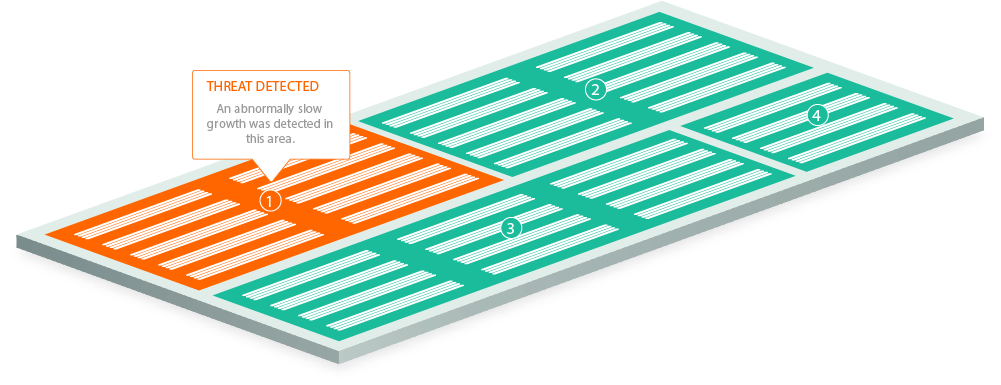
\includegraphics[width=1\linewidth]{vis_pers_lowlevel}
  \caption{Visualization work for the FitoAgro project under development.}
  \label{fig:vis_pers_lowlevel}
\end{figure}

More on the application in chapter \ref{sec:mobile_web_app}.

\section{Mobile and Web Applications} % (fold)
\label{sec:mobile_web_app}

Mobile and Web Applications are common ways to present the user with an interface to the server.

For this chapter, we consider two different use cases for the application usage:

\begin{itemize}
	\item The farmer is performing biological observations on one of his fields.
	\item The farmer is checking the state of his field and checking evolution of the pest overtime
\end{itemize}

While both use cases imply an interface for server communication, they will, most likely, be used in different contexts.

Ideally, web applications are for desktop/laptop usage. They can be responsive(readjust for any device size) but due to mobile-specific user interactions (scroll, swipe, etc.) and different design paradigms(for the two most common mobile operating systems: Apple and Android), native applications provide the user with a better interface that fits his device perfectly by following his operating system design guidelines. These rely on higher computing power (when compared to mobile devices) and bigger screens. This allows for more complex visualizations in general. 

On the other hand, mobile devices present a way for the user to interact with the system anywhere. Portability is obviously a major concern in this dissertation since farming fields are usually in remote locations. The biological observation data collection process involves movement since many trees have to be monitored throughout the field, and therefore, a small and portable device to upload information seems to be the ideal interface.

Organisations working in disparate domains are independently discovering patterns for building software that look the same. These systems are more robust, more resilient, more flexible and better positioned to meet modern demands.

These changes are happening because application requirements have changed dramatically in recent years. Only a few years ago a large application had tens of servers, seconds of response time, hours of offline maintenance and gigabytes of data. Today applications are deployed on everything from mobile devices to cloud-based clusters running thousands of multi-core processors. Users expect millisecond response times and 100\% uptime. Data is measured in petabytes. Today's demands are simply not met by yesterday’s software architectures.

The \textit{Reactive Manifesto} presents a coherent approach to systems architecture that fulfils present requirements. Systems built as Reactive Systems are more flexible, loosely-coupled and scalable. This makes them easier to develop and amenable to change. They are significantly more tolerant of failure and when failure does occur they meet it with elegance rather than disaster. Reactive Systems are highly responsive, giving users effective interactive feedback.

In general, Reactive systems are:

\begin{description}
	\item [Responsive] The system responds in a timely manner if at all possible. Responsiveness is the cornerstone of usability and utility, but more than that, responsiveness means that problems may be detected quickly and dealt with effectively. Responsive systems focus on providing rapid and consistent response times.
	\item [Resilient] The system stays responsive in the face of failure. This applies not only to highly available, mission-critical systems — any system that is not resilient will be unresponsive after a failure. Resilience is achieved by replication, containment, isolation and delegation.
	\item [Elastic] The system stays responsive under varying workload. Reactive Systems can react to changes in the input rate by increasing or decreasing the resources allocated to service these inputs. This implies designs that have no contention points or central bottlenecks.
	\item [Message Driven] Reactive Systems rely on asynchronous message-passing to establish a boundary between components that ensures loose coupling, isolation, and location transparency.
\end{description}

\subsection{Mobile Application}

Mobile Applications can be both native or cross-platform. Native Applications are built directly for the smartphone operating system while cross-platform are designed to fit more than one operating system.

There is a tradeoff between development time and performance. While cross-platform applications save time for the development team by forking developer code to both mobile standards, specific features may come with limited support and efficiency may not be as good as a native application.

\subsubsection{Native}

A native mobile app is a smartphone application that is coded in a specific programming language, such as \emph{Objective C} for \emph{iOS} or \emph{Java} for \emph{Android} operating systems. Native mobile apps provide fast performance and a high degree of reliability. They also have access to a phone's various devices, such as its camera and address book. In addition, users can use some apps without an internet connection. However, this type of app is expensive to develop because it is tied to one type of operating system, forcing the company that creates the app to make duplicate versions that work on other platforms.

\subsubsection{Hybrid or Cross-Platform}

This type of application has cross-platform compatibility but can still access a phone’s hardware. It is developed using platforms such as \emph{Sencha}, \emph{PhoneGap} or \emph{Mosync}. These were the usual approach for small teams developing for both platforms since they cut the development time in nearly half.

\subsubsection{React Native - The Best of both worlds}

Using the usual web development methodology, React Native inherited its component-based architecture from ReactJS (The predecessor and web version of React). Making use of the usual Model-View-Controller (\emph{MVC}) development pattern, this technology presents the developer with the ability to program the application once but export auto-generated native code for all the commercial operating systems: \emph{Windows Phone}, \emph{Android} and \emph{iOS}. This seems to be the modern approach of most development teams, migrating their mobile applications to React Native. The only technology that surpases \emph{React Native} in terms of performance (even though it is a minor gain) and extensibility is directly building native applications. 

\subsection{Web Application}

Web Applications, just like mobile, serve the interface to the user so that he is able to reach the computations from the server. In this subsection, some technologies are presented, discussed and compared.

\subsubsection{React}

As previously mentioned, \emph{React} is an open-source \emph{Javascript} component-based \emph{MVC}(Model-View-Controller) architecture for \emph{frontend}, made by \emph{Facebook}. \emph{React} makes it painless to create interactive UIs. Designing simple views for each state in the application, React will efficiently update and render just the right components when data changes. With components in Javascript, React renders possible the creation of a rich mobile User Interface (\textit{UI}) from declarative components.

Since component logic is written in JavaScript instead of templates, rich data can easily be passed through the app and keep state out of the \textit{DOM} (Domain Object Model).

\subsubsection{Angular}

\emph{Angular} (commonly referred to as "Angular 2+") is a \emph{TypeScript}-based open-source front-end web application platform led by the \emph{Angular} Team at \emph{Google} and by a community of individuals and corporations. \emph{Angular} is a complete rewrite from the same team that built \emph{AngularJS}.

The main difference between \emph{Angular} and \emph{React} for the web is probably the development speed. \emph{Angular} is much easier to set up and develop on, since most frontend patterns and utilities are already built-in as modules that can be imported. 

The performance is probably inferior to \emph{React}'s due to its life cycle (a continuous loop where the application looks for changes, and re-renders needed components when doing so). This is a problem for extensive applications, fast-changing \emph{DOM}s (realtime applications) but should not present a problem in this dissertation domain.


